\begin{figure}[ht]
\centering
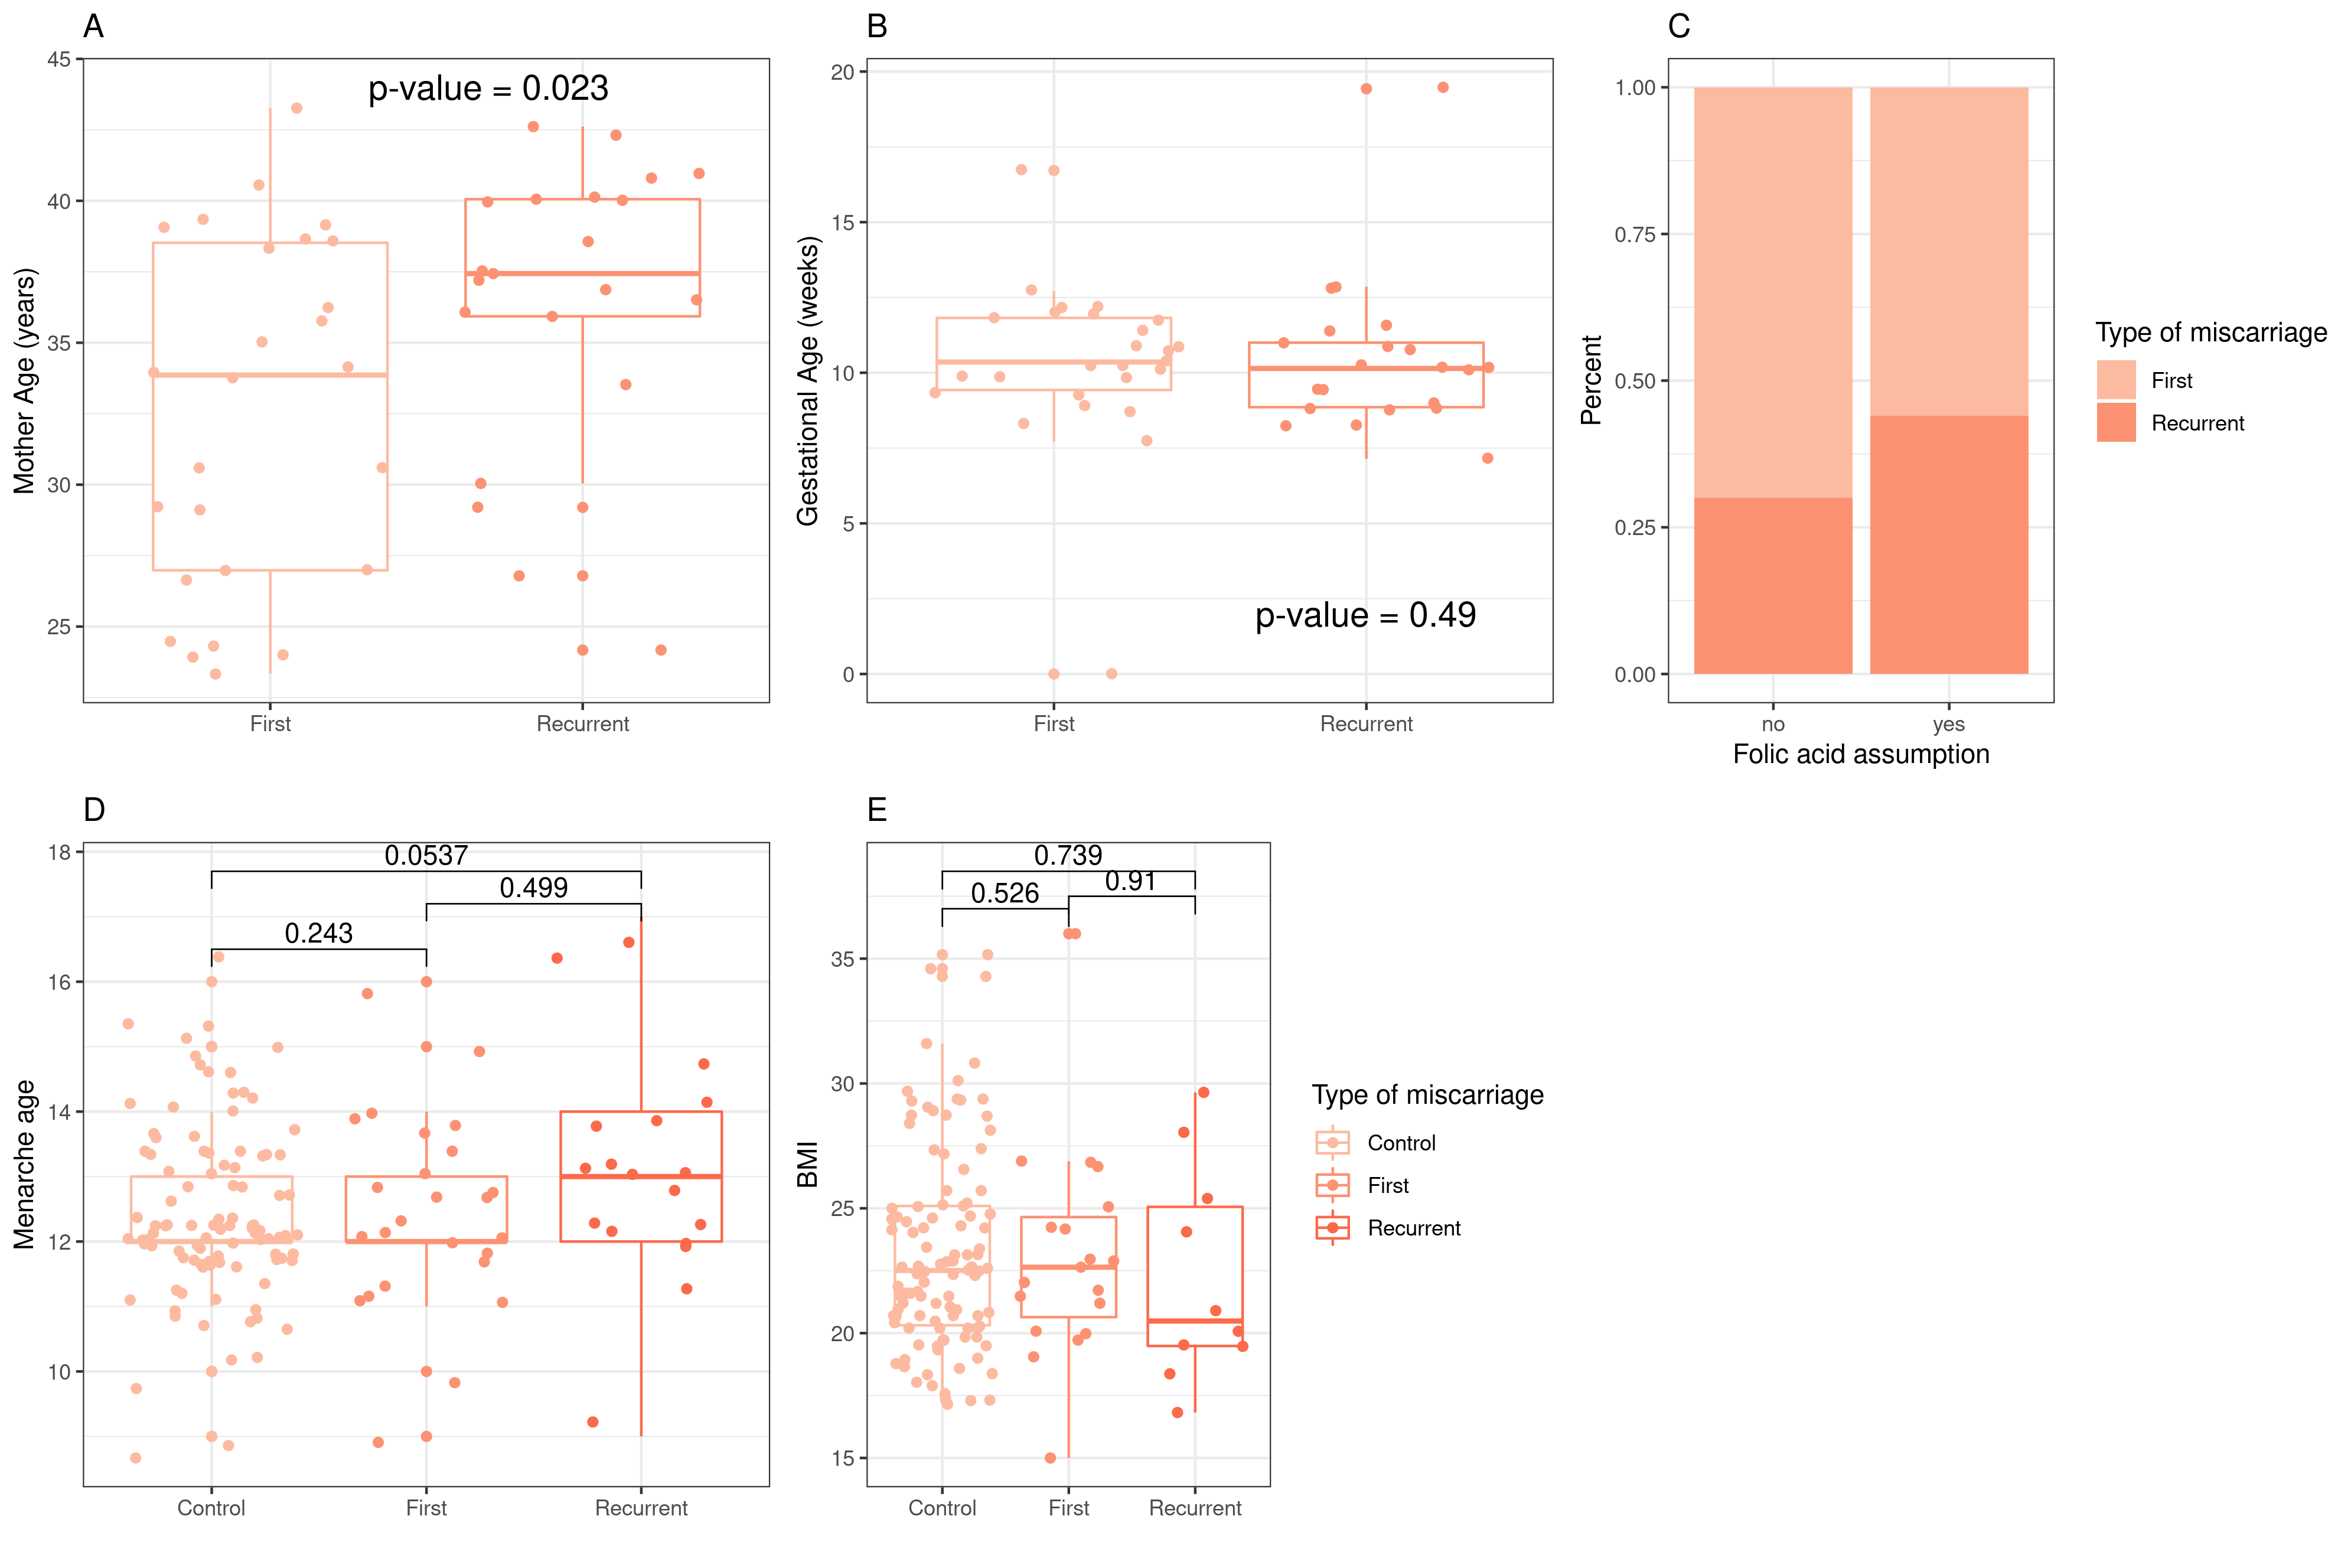
\includegraphics[width=\linewidth]{fig/panel_stats.png}
\caption{\textbf{Features of the embryo's mothers.} \textbf{(A)} Median age of the mother at the event is XX and XX for first and recurrent miscarriages, with no significant difference. \textbf{(B)} Gestational age at the time of the pregnancy termination range from X to X weeks with no significant difference between first and recurrent cases.  \textbf{(C)} Folic acid intake. Range of values of menarche age \textbf{(D)} and Body Mass Index \textbf{(E)} in embryo's mothers are not significantly different from a control set of mothers undergoing voluntary termination of pregnancy.}
\label{fig:embryostats}
\end{figure}

\begin{figure}[ht]
    \centering
    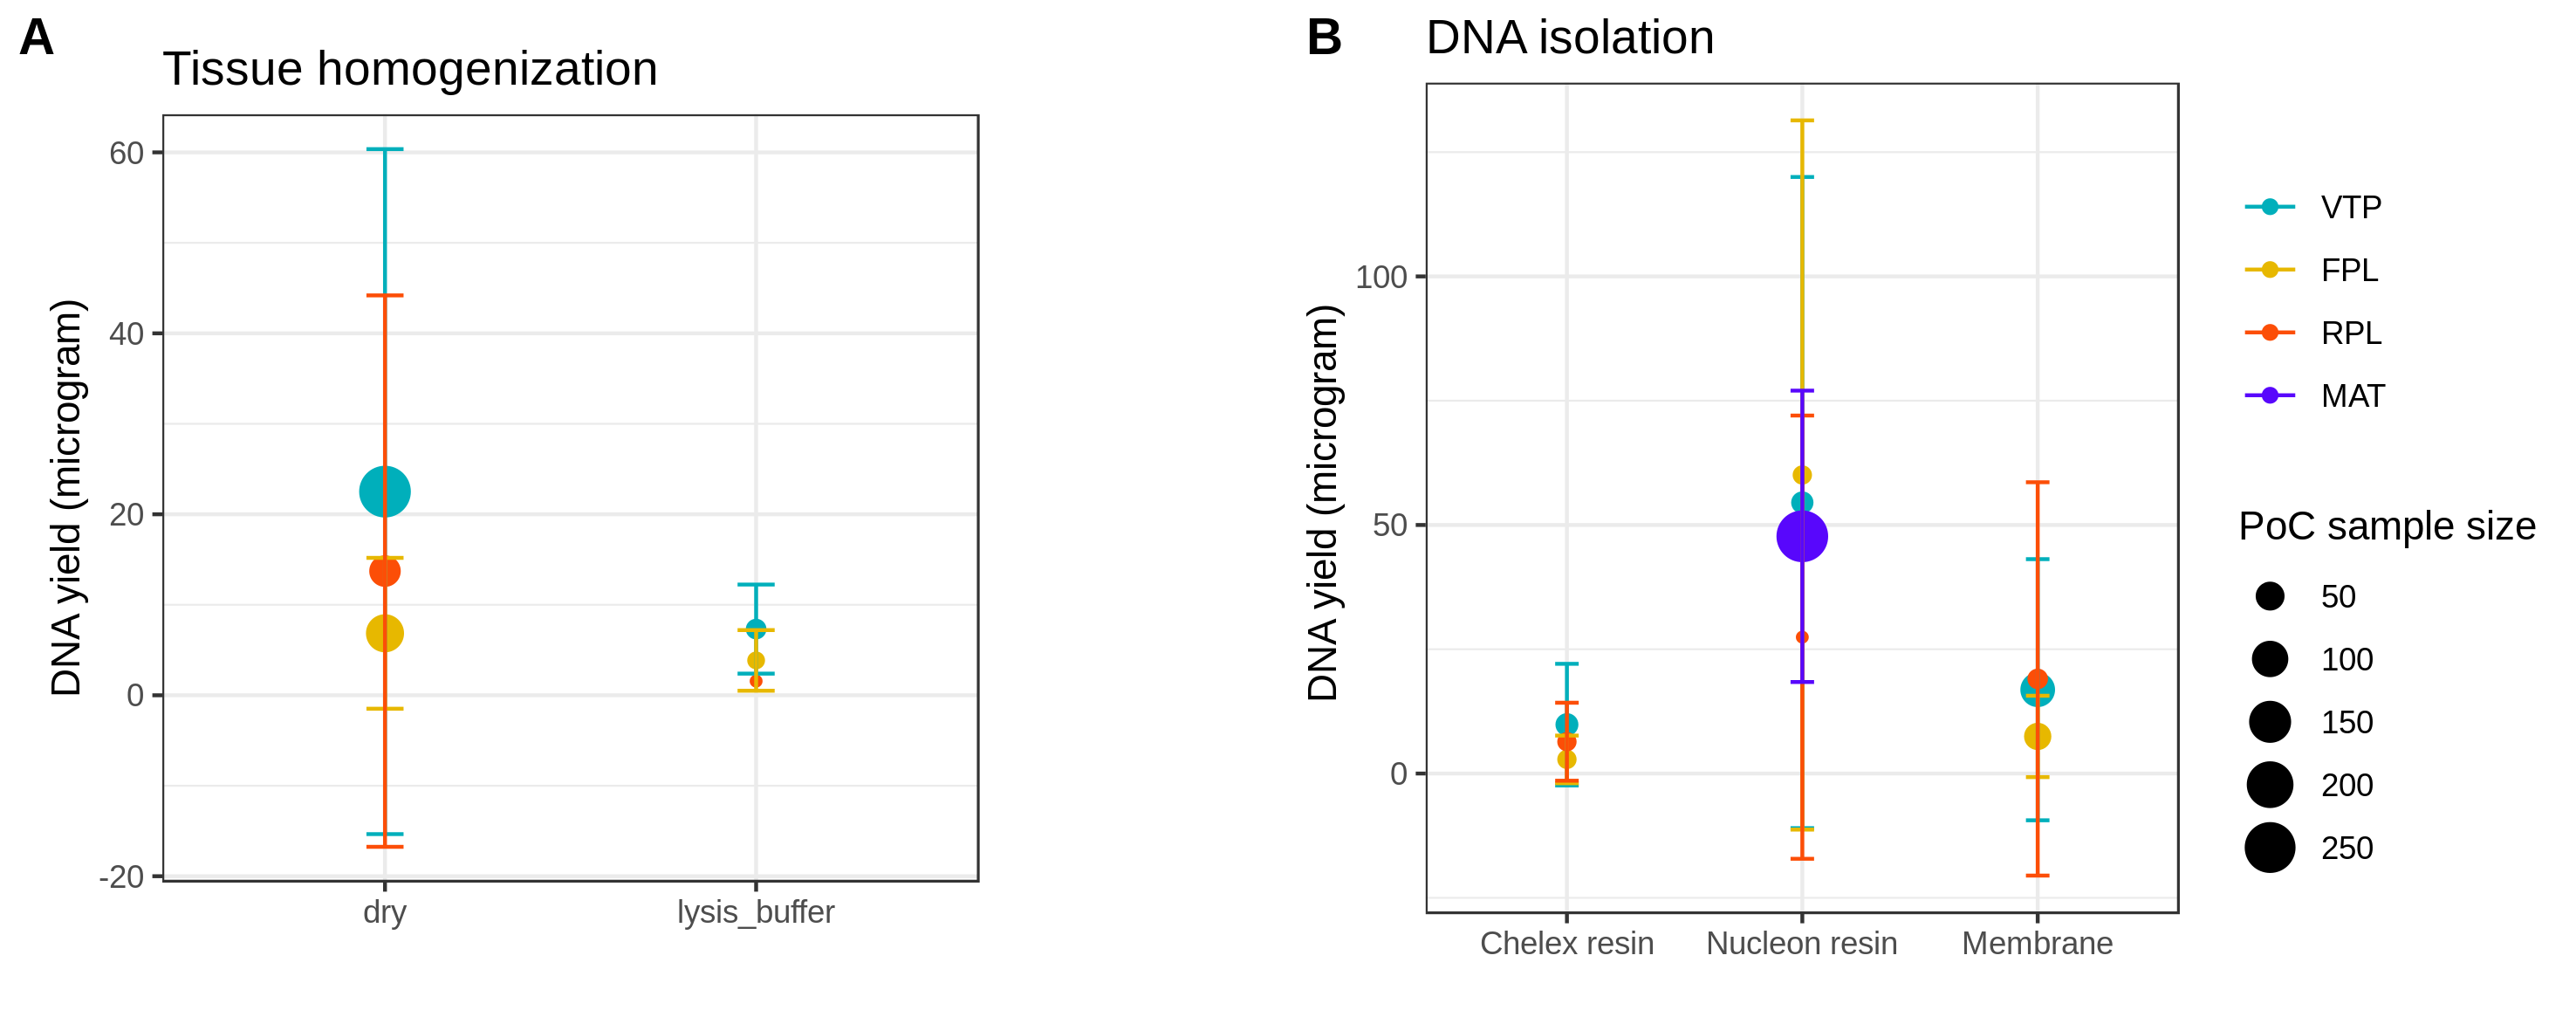
\includegraphics[width= 14 cm, high= 16cm]{fig/panelDNA.png}
    \caption{\textbf{Optimization of tissue homogenization and DNA extraction.} We do not observe significant difference between two methods of tissue homogenization (\textbf{A}), and three methods of DNA isolation (\textbf{b}) apart form a slightly higher range of yield for one type of resin. VTP: voluntary pregnancy termination;  FPL: first pregnancy loss; RPL:recurrent pregnancy loss;  MAT: maternal bllod; PoC: product of conception.}
    \label{fig:dna}
\end{figure}

\begin{figure}[ht]
    \centering
    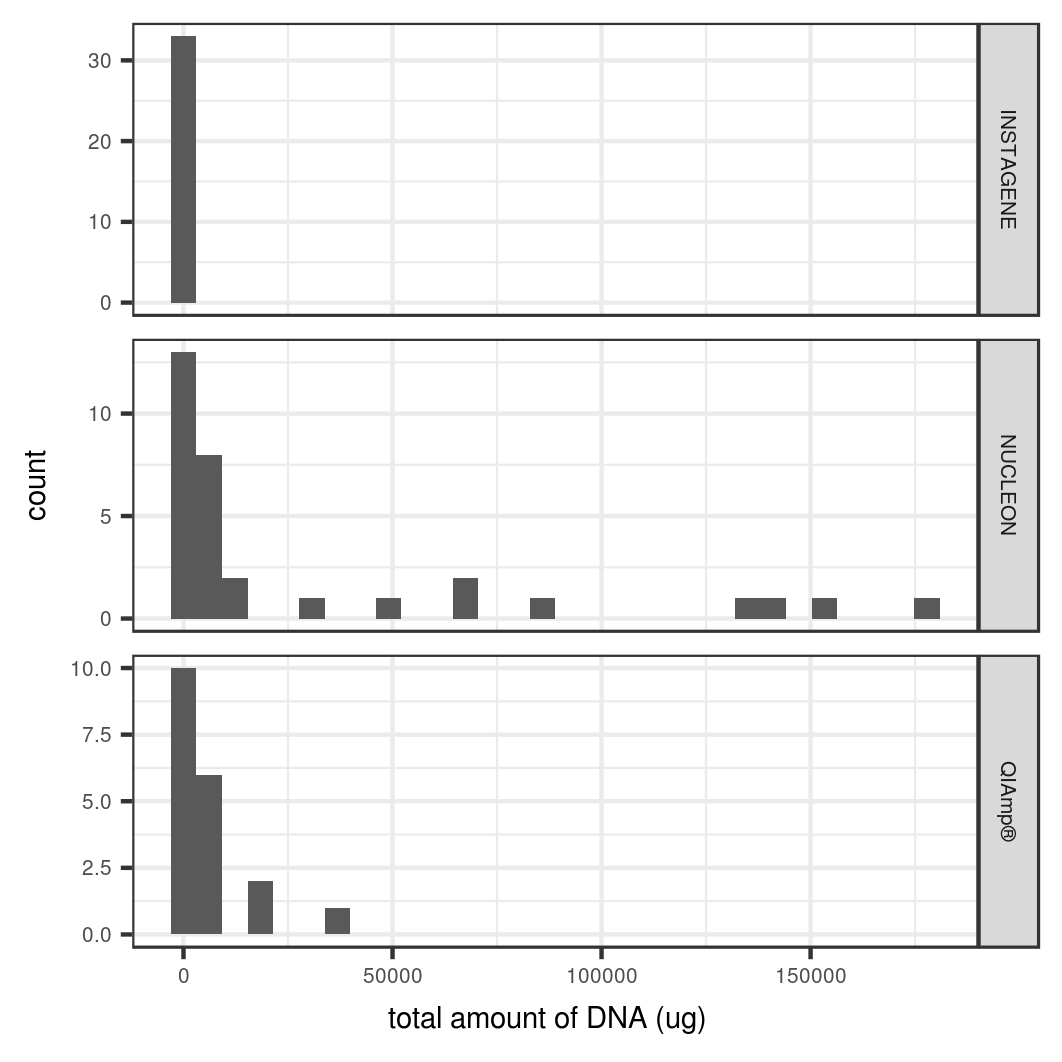
\includegraphics[width= 14 cm, high= 16cm]{fig/totaldna_bykit.png}
    \caption{\textbf{Yeld of DNA extraction form chorionic villi by extraction kit.} Distributions of total DNA as quantified using the  Qubit 2.0 Fluorometer} 
    \label{fig:dnayeld}
\end{figure}

\begin{figure}[ht]
    \centering
    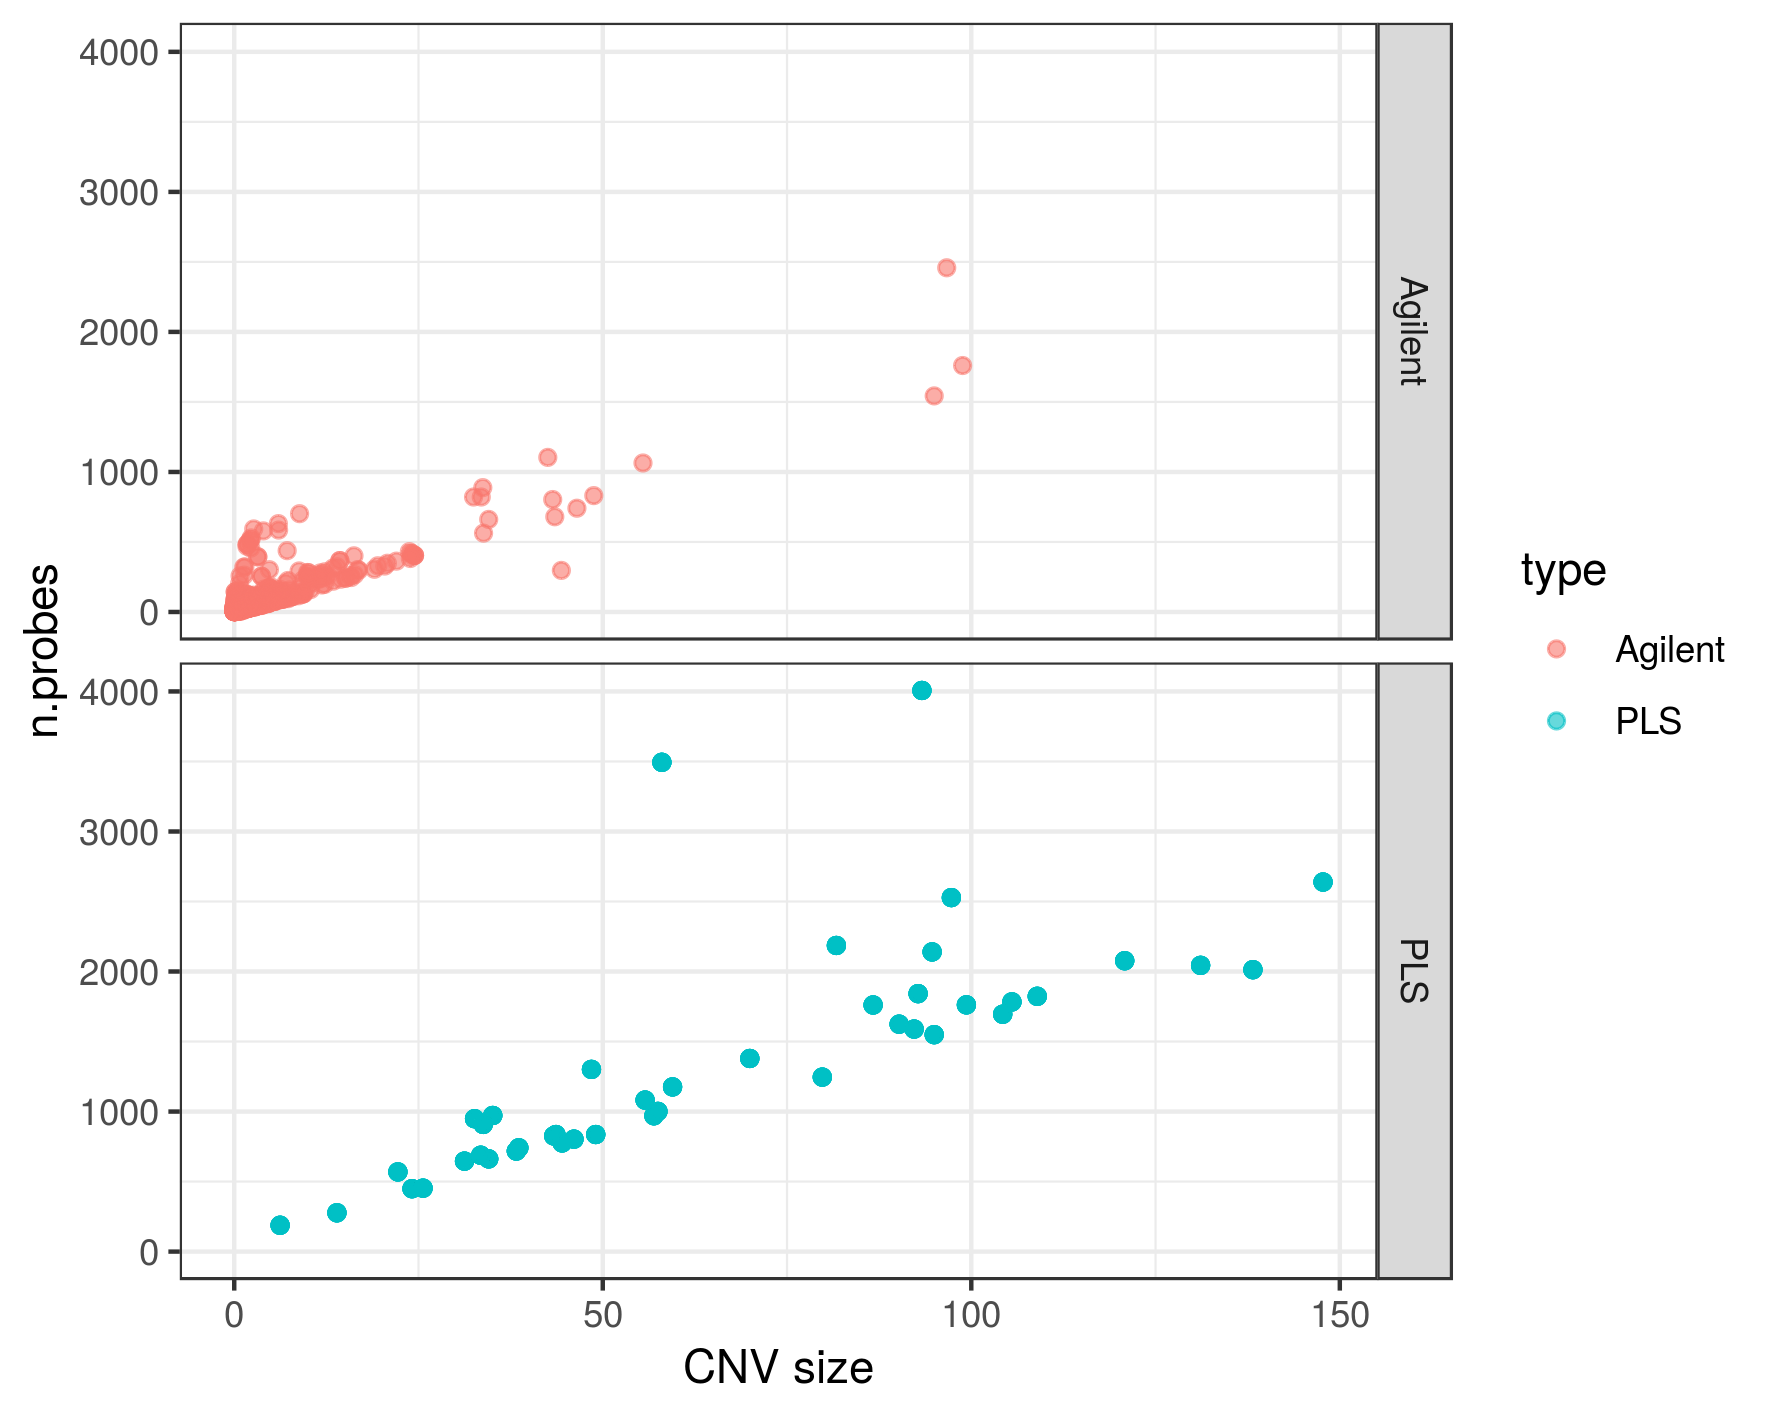
\includegraphics[width= 14 cm, high= 16cm]{fig/cnvCallComparison.png}
    \caption{\textbf{Copy number variant detection.} Comparison of calls made by the Agilent software and the penalized least square method implemented in the copynumber R package \cite{nilsen2012copynumber}} 
    \label{fig:cnvmethods}
\end{figure}